%\newcounter{alg:non-fifo:lines}
\begin{algo}[!ht]
\caption{SALSA implementation of SCPool: Data Structures.} 
\label{alg:non-fifo-ds}
%\scriptsize
\begin{minipage}[t]{0.48\textwidth}
\begin{distribalgo}[1]
\setcounter{ALC@line}{\value{alg:non-fifo:lines}}
\smallskip

\INDENT {{\bf Chunk type}}
	\STATE Task[CHUNK\_SIZE] tasks 
  \STATE int owner \comment {owner's consumer id}
\ENDINDENT

\INDENT {{\bf Node type}}
  \STATE Chunk c; initially $\bot$
  \STATE int idx; initially -1
  \STATE Node next; 
\ENDINDENT

\setcounter{alg:non-fifo:lines}{\value{ALC@line}} % store the line number
\end{distribalgo}
\end{minipage}%
%
\hfill
%
\begin{minipage}[t]{0.48\textwidth}
%
\begin{distribalgo}[1]
\setcounter{ALC@line}{\value{alg:non-fifo:lines}}
\smallskip

\INDENT {{\bf SALSA per consumer data structure}:}
  \STATE int consumerId
  \STATE List\tup{Node}[] chunkLists \comment {one list per producer + extra list for stealing (every list is single-writer multi-reader)} 
  \STATE Queue\tup{Chunk} chunkPool \comment {pool of spare chunks}
  \STATE Node currentNode, initially $\bot$ \comment {current node to work with} 
\ENDINDENT

\setcounter{alg:non-fifo:lines}{\value{ALC@line}}
\end{distribalgo}
\end{minipage}
\end{algo}

%\begin{wrapfigure}{l}{0.5\textwidth}
%  \vspace{-20pt}
%  \begin{center}
%    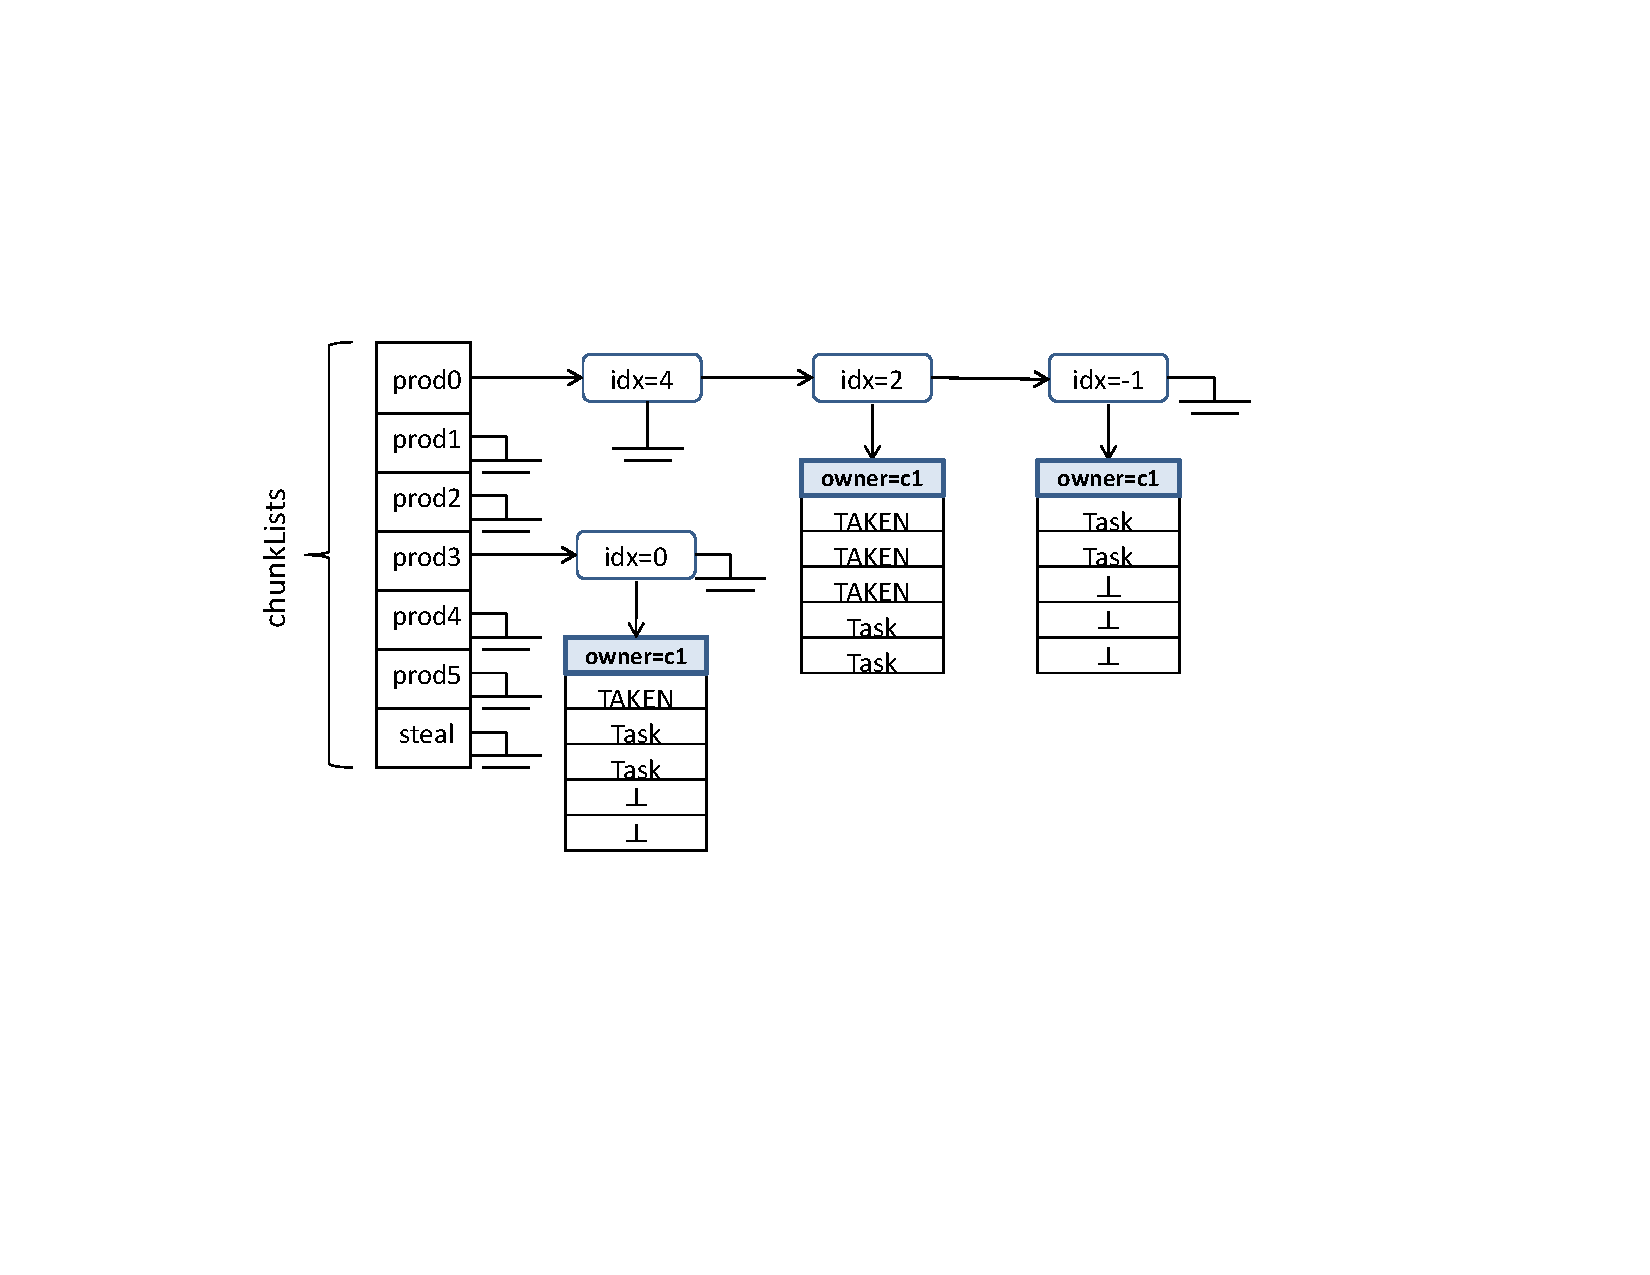
\includegraphics[width=0.48\textwidth]{figures/salsa-struct}
%  \end{center}
%  \vspace{-20pt}
%  \caption{\footnotesize{Chunk lists in SALSA single consumer pool implementation. Tasks are kept in chunks, which are 
%	    organized in per-producer lists; an additional list is reserved for stealing. Each list can be modified 
%	    by the corresponding producer only. The only process that is allowed to retrieve tasks from a chunk is 
%	    the owner of that chunk (defined by the ownership flag). A Node's index corresponds to the latest task taken from the chunk
%	    or the task that is about to be taken by the current chunk owner. 
%	    }}
%  \vspace{-10pt}
%  \label{fig:salsa-struct}
%\end{wrapfigure}

\begin{figure}[htb]
	\centering
	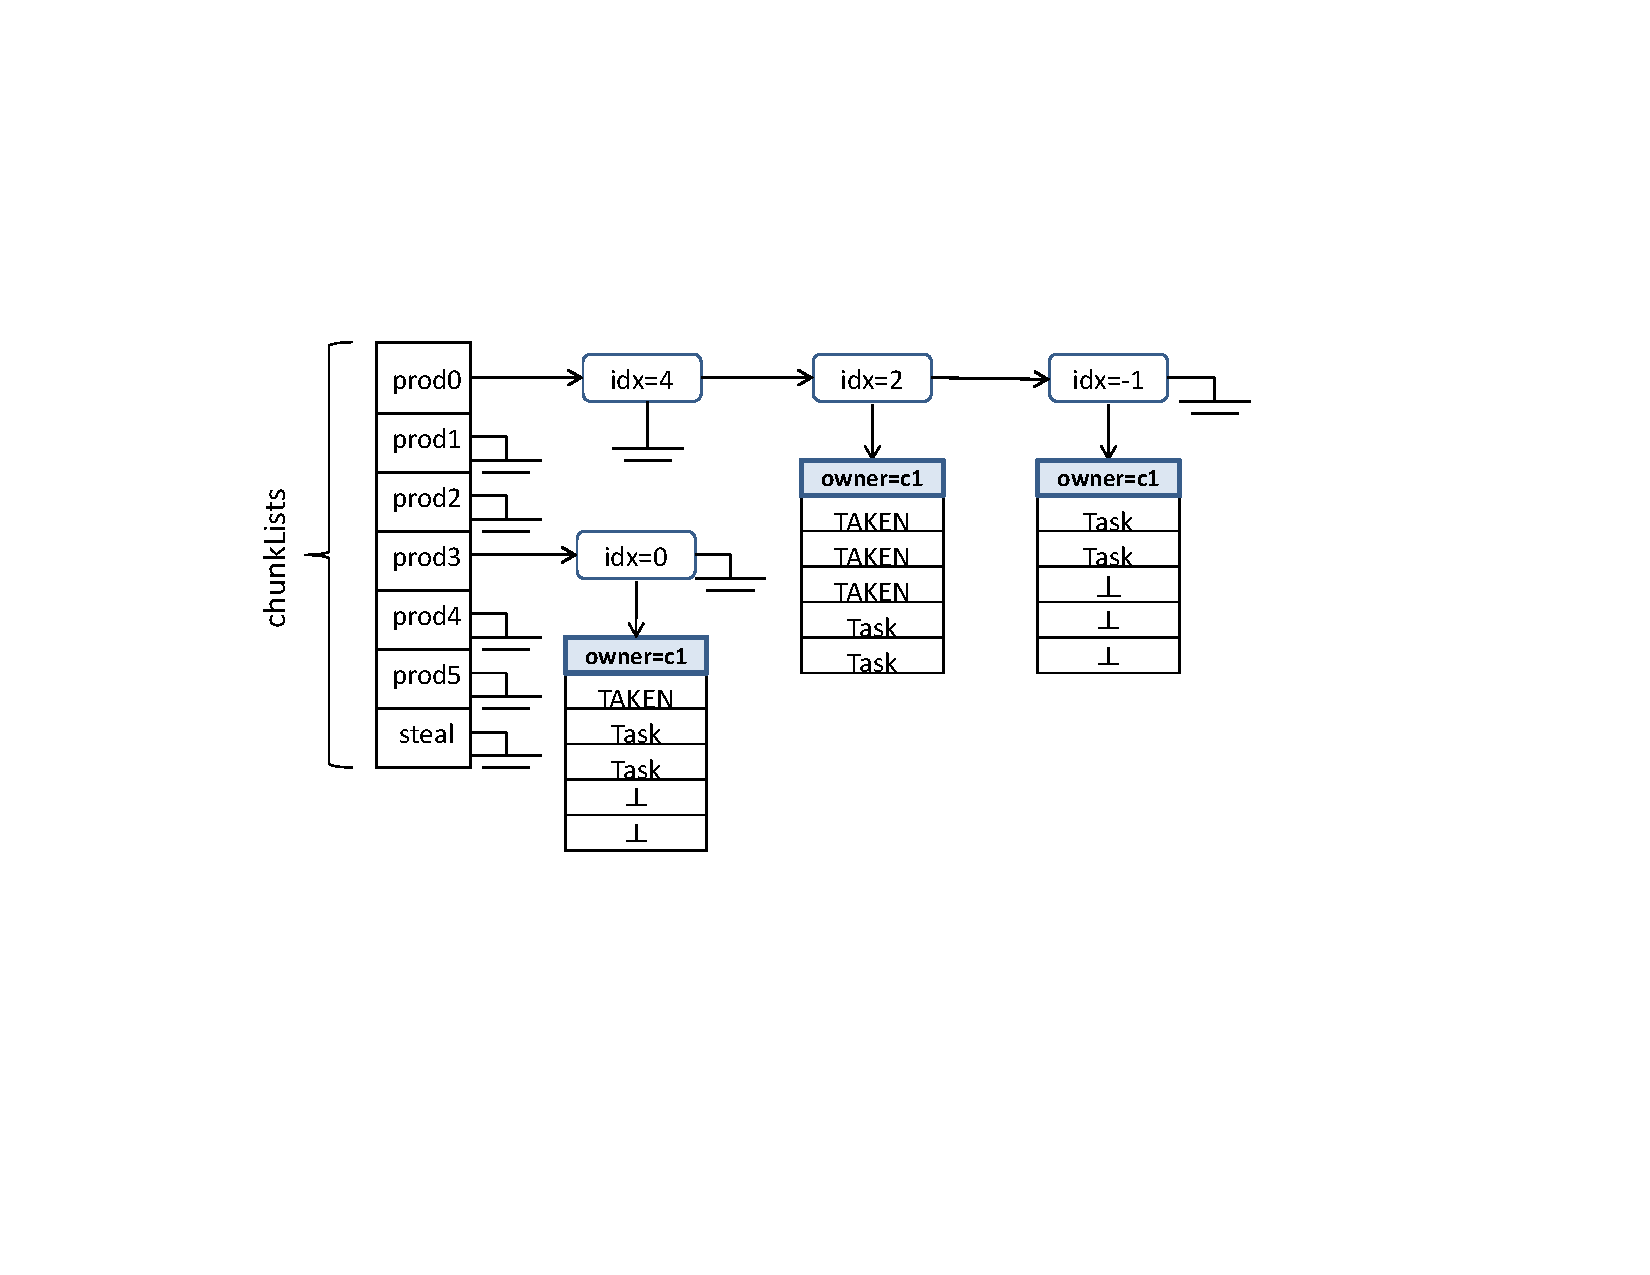
\includegraphics[width=0.5\textwidth]{figures/salsa-struct}
	\vspace{-10pt}
	\caption{
	    \footnotesize{Chunk lists in SALSA single consumer pool implementation. Tasks are kept in chunks, which are 
	    organized in per-producer lists; an additional list is reserved for stealing. Each list can be modified 
	    by the corresponding producer only. The only process that is allowed to retrieve tasks from a chunk is 
	    the owner of that chunk (defined by the ownership flag). A Node's index corresponds to the latest task taken from the chunk
	    or the task that is about to be taken by the current chunk owner. 
	    }}
	\label{fig:salsa-struct}
	\vspace{-5pt}
\end{figure}

The SALSA data structure of a consumer $c_i$ is described in Algorithm~\ref{alg:non-fifo-ds} and partially depicted in Figure~\ref{fig:salsa-struct}. 
%We describe the implementation of a SALSA SCPool of some consumer $c_i$.
%Its data structures are described in Algorithm~\ref{alg:non-fifo-ds} and partially depicted in Figure~\ref{fig:salsa-struct}. 
The tasks inserted to SALSA are kept in chunks, which are organized in per-producer chunk lists. Only the producer mapped to a given list can insert a task to any chunk in that list. Every chunk is owned by a single consumer whose id is kept in the \emph{owner} field of the chunk.
The owner is the only process that is allowed to take tasks from the chunk; if another process wants to take a task from the chunk, it should first steal the chunk and change its ownership. 
%The owner of a chunk residing at $c_i$'s SCPool is $c_i$ itself, unless that chunk is being stolen. 
A task entry in a chunk is used at most once. Its value is $\bot$ before the task is inserted, and TAKEN after it has been consumed.

The per-producer chunk lists are kept in the array \emph{chunkLists} (see Figure~\ref{fig:salsa-struct}), where \emph{chunkLists[j]} keeps a list of chunks with tasks inserted by producer $p_j$. In addition, the array has a special entry \emph{chunkLists[steal]}, holding chunks stolen by $c_i$. Every list has a single writer who can modify the list structure (add or remove nodes): \emph{chunkLists[j]}'s modifier is the producer $p_j$, while \emph{chunkLists[steal]}'s modifer is the SCPool's owner. 
The nodes of the used chunks are lazily reclaimed and removed by the list's owner. For brevity, we omit the linked list manipulation functions from the pseudo-code bellow. Our single-writer lists can be implemented without synchronization primitives, similarly to the single-writer linked-list in~\cite{Michael:2004:HPS:987524.987595}.
In addition to holding the chunk, a node keeps the index of the latest taken task in that chunk, this index is then used for chunk stealing as we show in Section~\ref{alg-stealing}. 

Safe memory reclamation is provided by using hazard pointers~\cite{Michael:2004:HPS:987524.987595} both for nodes and for chunks.
The free (reclaimed) chunks in SALSA are kept at per-consumer \emph{chunkPools} implemented by lock-free Michael-Scott queues~\cite{Michael:1996:SFP:248052.248106}. As we show in Section~\ref{alg-pools}, the chunk pools serve two purposes: 1) efficient memory reuse and 2) producer-based load balancing.  	